
\subsection{Aufbau}
\label{sec:Aufbau}

\begin{figure}[H]
\centering
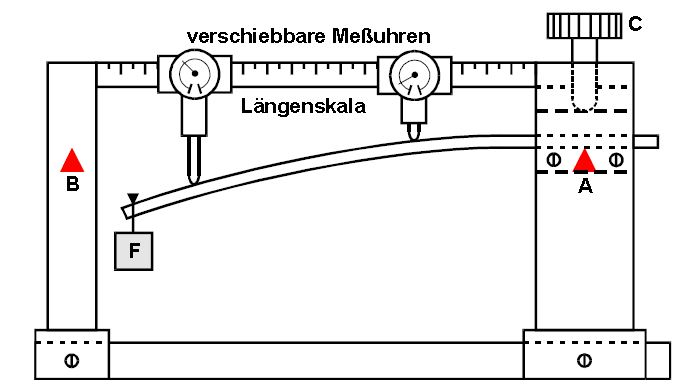
\includegraphics[width=\linewidth-30pt,height=\textheight-30pt,keepaspectratio]{Text/Bilder/Aufbau.png}
\caption{Versuchsanordnung zur Ausmessung einer Beugungsfigur \cite[36]{sample}.}
\label{fig:aufbau}
\end{figure}

Der in Abbildung \ref{fig:aufbau} dargestellte Aufbau besteht aus einem Laser, einem verschiebbaren Spalt, sowie einem Verschiebereiter mit Photoelement mit Abstand $L$ zum Laser.
Das Photoelement ist mit einem Amperemeter gekoppelt, mit dessen Hilfe die Intensität des Lichtes abgegriffen werden kann.
\section{Durchführung}
\label{sec:Durchführung}
Zunächst wird der Abstand $L$ zwischen Laser und Photodetektor gemessen.  Daraufhin werden Amperemeter und Photodetektor eingeschaltet und der
Dunkelstrom $I_\text{d}$ abgelesen. Anschließend wird ein Einzelspalt vor den Laser gesetzt, sodass Interferenzmuster auftreten.
Das Photoelement wird zwischen den Nebenmaxima 1. Ordnung verschoben, wobei 50 Messwerte aufgenommen werden.
Dies wird für zwei Doppelspalte wiederholt, wobei dort das Photoelement zwischen den Nebenmaxima 2. Ordnung verschoben wird.
